% make sure not a repeat header!
\subsection{Getting started in EA}
\visHeader
\hypertarget{static:starting vis}{}

You can begin modeling Leitner's Box in two different ways. You can either continue in the same workspace as the Part I demo by opening the previous
\texttt{demo.eap} file in EA, initializating a new diagram and working within that space, or you can start this project with a clean slate by going to ``New
Metamodel Project,'' choosing to start a new visual project (without the demo specifications) (Fig.~\ref{fig:new_visModel}), and opening that empty
\texttt{.eap} file. This handbook has assumed you prefer the latter, which is reflected in the screenshots. If you use the previous file, please note that the
steps are exactly the same, but our package explorers may not match exactly. Keep a sharp eye out for footnotes which will explain the few differences.

\begin{figure}[htbp]
	\centering
  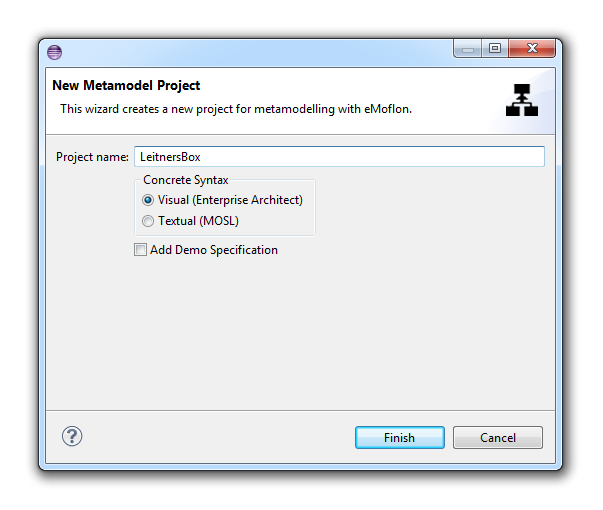
\includegraphics[width=0.75\textwidth]{eclipse_newMetamodelVisualPlain}
	\caption{Starting a new visual project}
	\label{fig:new_visModel}
\end{figure}

\newpage
\begin{itemize}
\item[$\blacktriangleright$] From EA, select your working set and press the ``Add a Package'' button (Fig.~\ref{fig:new_package})\footnote{If using the previous
files, you won't have the \texttt{eMoflon Languages} package, since all the needed files were included in \texttt{Demo}. For this simple example, we won't be
using all the features of eMoflon, so this limited collection will suffice.}.

\begin{figure}[htbp]
	\centering
  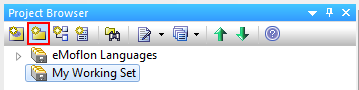
\includegraphics[width=0.5\textwidth]{ea_addPackage}
	\caption{Add a new package to \texttt{MyWorkingSet}}
	\label{fig:new_package}
	\vspace{0.5cm}
\end{figure}

\vspace{1.0cm}

\item[$\blacktriangleright$] In the dialogue that pops up (Fig.~\ref{fig:new_package_name}), enter `Learning\-Box\-Language' as the name of the new package.
Make sure \texttt{Class View} is selected, and click \texttt{OK}.

\begin{figure}[htbp]
	\centering
    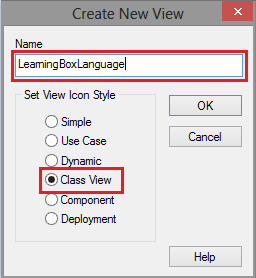
\includegraphics[width=0.33\textwidth]{ea_namePackage.png}
	\caption{Enter the name of the new package}
	\label{fig:new_package_name}
\end{figure}
\FloatBarrier

\vspace{1.0cm}

\item[$\blacktriangleright$] Your \texttt{Project Browser} should now resemble Fig.~\ref{fig:new_package_completed}.

\begin{figure}[htbp]
	\centering
  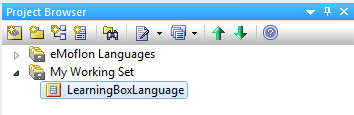
\includegraphics[width=0.5\textwidth]{ea_newPackage}
	\caption{State after creating the new package.}
	\label{fig:new_package_completed}
\end{figure}
\FloatBarrier

\clearpage
\item[$\blacktriangleright$] Now create a ``New Diagram'' (Fig.~\ref{fig:diagram}).

\begin{figure}[htbp]
	\centering
  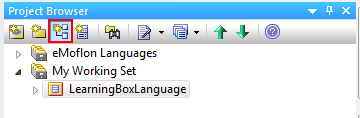
\includegraphics[width=0.5\textwidth]{ea_addDiagram}
	\caption{Add a diagram.}
	\label{fig:diagram}
\end{figure}
\FloatBarrier

\item[$\blacktriangleright$] In the dialogue that appears, (Fig.~\ref{fig:diagram_type}), choose \texttt{eMoflon Ecore Diagrams}, then press \texttt{OK}. The
name will be automatically created.

\begin{figure}[htbp]
	\centering
  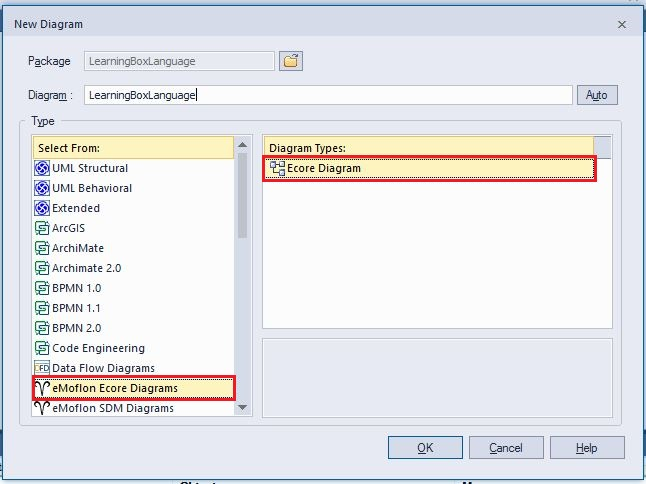
\includegraphics[width=0.8\textwidth]{ea_chooseDiagramType}
	\caption{Select the ecore diagram type}
	\label{fig:diagram_type}
\end{figure}
\FloatBarrier

 
\item[$\blacktriangleright$] After creating the new diagram, your  \texttt{Project Browser} should now resemble Fig.~\ref{fig:diagram_completed}. You'll notice
that your \texttt{LearningBoxLanguage} package transformed into a container. This will now be the source location for any and all diagrams, the place where
all your generated files are derived.

\begin{figure}[htbp]
	\centering
  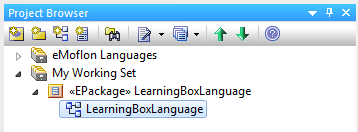
\includegraphics[width=0.5\textwidth]{ea_afterDiagramState}
	\caption{State after creating diagram}
	\label{fig:diagram_completed}
\end{figure}
\FloatBarrier

\newpage

\item[$\blacktriangleright$] To finalize the initalization of your metamodel, export your project to Eclipse\footnote{If unsure how to perform this step, please
refer to Section 2.1 in Part I.}, then refresh your \texttt{Package Explorer}. A new \texttt{Other Projects} node\footnote{If you do not have the two distinct
nodes, make sure your ``Top Level Elements'' are set to \texttt{Working Sets}} should have appeared containing your adapted \texttt{Epackage}
(Fig.~\ref{fig:init_import}). You can see the that a \texttt{LearningBoxLanguage.ecore} file has been generated, and placed in ``model.'' This is the graph of
your metamodel that will adhere to all future types and restrictions you create.

\vspace{0.5cm}

\begin{figure}[htbp]
	\centering
  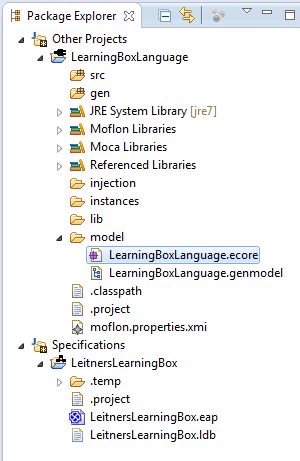
\includegraphics[width=0.5\textwidth]{eclipse_initExport}
	\caption{Inital import to Eclipse}
	\label{fig:init_import}
\end{figure}
\FloatBarrier

\vspace{0.5cm}

\item[$\blacktriangleright$] If you'd like to review the overall project structure, the purposes of certain files and folders, read Section 4 from
Part~I\footnote{\downLink} of this handbook. Otherwise, click to learn how to declare your classes and attributes.

\fancyfoot[R]{$\triangleright$ \hyperlink{static:classes vis}{Next}}
\end{itemize}
